\documentclass[12pt]{article}
\usepackage[utf8]{inputenc}
\usepackage{datetime}
\usepackage{cite}
\usepackage{url}
\usepackage[numbers]{natbib}
\usepackage{lscape}
\usepackage{tikz}
\usetikzlibrary{arrows}

\newdateformat{monthyeardate}{\monthname[\THEMONTH], \THEYEAR}

\title{History of Project Teams at Cornell}
\author{Alex Renda (adr74)}
\date{\monthyeardate\today}

\begin{document}

\maketitle

\section{Introduction}

\section{Background}

\section{Timeline}

\begin{landscape}
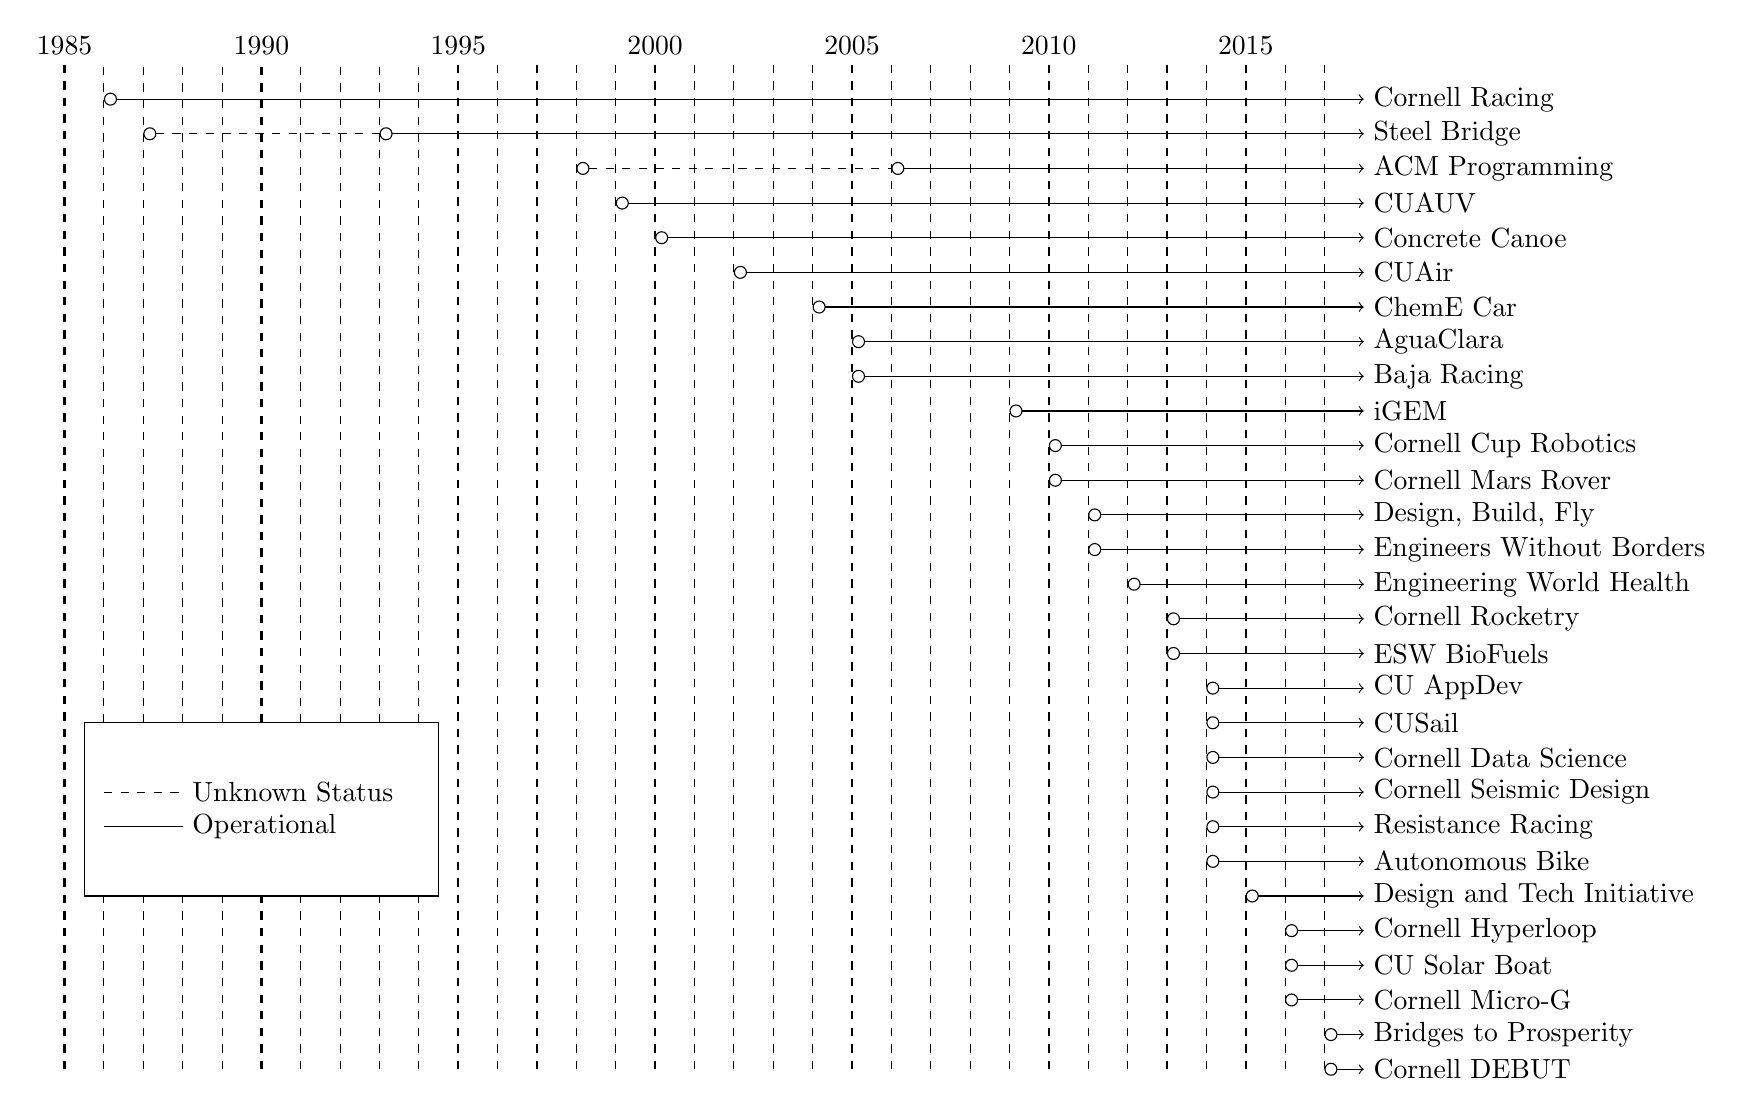
\begin{tikzpicture}[x=0.5cm, y=0.44cm]

\draw[dashed] (1, 8) -- (3, 8);
\node[right] at (3, 8) {Unknown Status};

\draw (1, 7) -- (3, 7);
\node[right] at (3, 7) {Operational};

\draw (0.5,5) -- (0.5,10) -- (9.5,10) -- (9.5,5) -- (0.5,5);


\node[above] at (0, 29) {1985};
\draw[dashed, thick] (0, 0) -- (0, 29);
\draw[dashed] (1, 0) -- (1, 5);
\draw[dashed] (1, 10) -- (1, 29);
\draw[dashed] (2, 0) -- (2, 5);
\draw[dashed] (2, 10) -- (2, 29);
\draw[dashed] (3, 0) -- (3, 5);
\draw[dashed] (3, 10) -- (3, 29);
\draw[dashed] (4, 0) -- (4, 5);
\draw[dashed] (4, 10) -- (4, 29);
\node[above] at (5, 29) {1990};
\draw[dashed, thick] (5, 0) -- (5, 5);
\draw[dashed, thick] (5, 10) -- (5, 29);
\draw[dashed] (6, 0) -- (6, 5);
\draw[dashed] (6, 10) -- (6, 29);
\draw[dashed] (7, 0) -- (7, 5);
\draw[dashed] (7, 10) -- (7, 29);
\draw[dashed] (8, 0) -- (8, 5);
\draw[dashed] (8, 10) -- (8, 29);
\draw[dashed] (9, 0) -- (9, 5);
\draw[dashed] (9, 10) -- (9, 29);
\node[above] at (10, 29) {1995};
\draw[dashed, thick] (10, 0) -- (10, 29);
\draw[dashed] (11, 0) -- (11, 29);
\draw[dashed] (12, 0) -- (12, 29);
\draw[dashed] (13, 0) -- (13, 29);
\draw[dashed] (14, 0) -- (14, 29);
\node[above] at (15, 29) {2000};
\draw[dashed, thick] (15, 0) -- (15, 29);
\draw[dashed] (16, 0) -- (16, 29);
\draw[dashed] (17, 0) -- (17, 29);
\draw[dashed] (18, 0) -- (18, 29);
\draw[dashed] (19, 0) -- (19, 29);
\node[above] at (20, 29) {2005};
\draw[dashed, thick] (20, 0) -- (20, 29);
\draw[dashed] (21, 0) -- (21, 29);
\draw[dashed] (22, 0) -- (22, 29);
\draw[dashed] (23, 0) -- (23, 29);
\draw[dashed] (24, 0) -- (24, 29);
\node[above] at (25, 29) {2010};
\draw[dashed, thick] (25, 0) -- (25, 29);
\draw[dashed] (26, 0) -- (26, 29);
\draw[dashed] (27, 0) -- (27, 29);
\draw[dashed] (28, 0) -- (28, 29);
\draw[dashed] (29, 0) -- (29, 29);
\node[above] at (30, 29) {2015};
\draw[dashed, thick] (30, 0) -- (30, 29);
\draw[dashed] (31, 0) -- (31, 29);
%\node[above] at (32, 29) {2017};
\draw[dashed] (32, 0) -- (32, 29);


% Cornell Racing: 1986
\node [right] at (33, 28) {Cornell Racing};
\draw[o->] (1, 28) -- (33, 28);

% Steel Bridge: 1987 -- 1993 - pres
\node [right] at (33, 27) {Steel Bridge};
\draw[dashed, o-] (2, 27) -- (8, 27);
\draw[o->] (8, 27) -- (33, 27);

% Cornell ACM Programming: 1998 -- 2006 - pres
\node [right] at (33, 26) {ACM Programming};
\draw[dashed, o-] (13, 26) -- (21, 26);
\draw[o->] (21, 26) -- (33, 26);

% CUAUV: 1999
\node [right] at (33, 25) {CUAUV};
\draw[o->] (14, 25) -- (33, 25);

% Concrete Canoe: 2000
\node [right] at (33, 24) {Concrete Canoe};
\draw[o->] (15, 24) -- (33, 24);

% CUAir: 2002
\node [right] at (33, 23) {CUAir};
\draw[o->] (17, 23) -- (33, 23);

% ChemE Car: 2004
\node [right] at (33, 22) {ChemE Car};
\draw[o->] (19, 22) -- (33, 22);

% AguaClara: 2005
\node [right] at (33, 21) {AguaClara};
\draw[o->] (20, 21) -- (33, 21);

% Baja Racing: 2005
\node [right] at (33, 20) {Baja Racing};
\draw[o->] (20, 20) -- (33, 20);

% iGEM: 2009
\node [right] at (33, 19) {iGEM};
\draw[o->] (24, 19) -- (33, 19);

% Cornell Cup Robotics: 2010
\node [right] at (33, 18) {Cornell Cup Robotics};
\draw[o->] (25, 18) -- (33, 18);

% Cornell Mars Rover: 2010
\node [right] at (33, 17) {Cornell Mars Rover};
\draw[o->] (25, 17) -- (33, 17);

% Design, Build, Fly: 2011
\node [right] at (33, 16) {Design, Build, Fly};
\draw[o->] (26, 16) -- (33, 16);

% Engineers Without Borders: 2011
\node [right] at (33, 15) {Engineers Without Borders};
\draw[o->] (26, 15) -- (33, 15);

% Engineering World Health: 2012
\node [right] at (33, 14) {Engineering World Health};
\draw[o->] (27, 14) -- (33, 14);

% Cornell Rocketry: 2013
\node [right] at (33, 13) {Cornell Rocketry};
\draw[o->] (28, 13) -- (33, 13);

% ESW Biofuels: 2013
\node [right] at (33, 12) {ESW BioFuels};
\draw[o->] (28, 12) -- (33, 12);

% CU AppDev: 2014
\node [right] at (33, 11) {CU AppDev};
\draw[o->] (29, 11) -- (33, 11);

% CUSail: 2014
\node [right] at (33, 10) {CUSail};
\draw[o->] (29, 10) -- (33, 10);

% Cornell Data Science: 2014
\node [right] at (33, 9) {Cornell Data Science};
\draw[o->] (29, 9) -- (33, 9);

% Cornell Seismic Design: 2014
\node [right] at (33, 8) {Cornell Seismic Design};
\draw[o->] (29, 8) -- (33, 8);

% Resistance Racing: 2014
\node [right] at (33, 7) {Resistance Racing};
\draw[o->] (29, 7) -- (33, 7);

% Autonomous Bike: 2014
\node [right] at (33, 6) {Autonomous Bike};
\draw[o->] (29, 6) -- (33, 6);

% Cornell Design and Tech Initiative: 2015
\node [right] at (33, 5) {Design and Tech Initiative};
\draw[o->] (30, 5) -- (33, 5);

% Cornell Hyperloop: 2016
\node [right] at (33, 4) {Cornell Hyperloop};
\draw[o->] (31, 4) -- (33, 4);

% CU Solar Boat: 2016
\node [right] at (33, 3) {CU Solar Boat};
\draw[o->] (31, 3) -- (33, 3);

% Cornell Micro-G: 2016
\node [right] at (33, 2) {Cornell Micro-G};
\draw[o->] (31, 2) -- (33, 2);

% Bridges to Prosperity: 2017
\node [right] at (33, 1) {Bridges to Prosperity};
\draw[o->] (32, 1) -- (33, 1);

% Cornell DEBUT: 2017
\node [right] at (33, 0) {Cornell DEBUT};
\draw[o->] (32, 0) -- (33, 0);

\end{tikzpicture}

%%% Local Variables:
%%% TeX-master: "report"
%%% End:
\end{landscape}

``The CUAUV team, as we know it today, was started by sophomores Serguei Vassilvitskii, Nidhi Kalra, Jack Chuang, and Walter Chang in September of 1999,''
\cite{noauthor_cuauv_2003}

``Cornell Racing is the "granddaddy" of engineering project teams, says Rebecca Macdonald, the Swanson Director of Engineering Student Project Teams at Cornell,''
\cite{klein_engineering_2015}

``Cornell’s Formula SAE Team was established in 1986.''
\cite{noauthor_cornell_2012}

Baja established in 2005:
\cite{noauthor_history_2017}

``Cornell participated in this competition as part of OpenLoop, a team of students from Cornell, Harvey Mudd College, University of Michigan, Northeastern, Memorial University of Newfoundland, and Princeton.  OpenLoop’s design for the pod prototype made it through the initial rounds, but the team was not able to build the pod prototype.

But in Fall 2016, Cornell Hyperloop broke off from OpenLoop, and is determined to win SpaceX 2018 Hyperloop Pod Competition in summer 2018.''
\cite{roseman_how_2017}

``While they couldn’t register immediately as a team, says Rebecca Macdonald, the Swanson Director of Engineering Student Project Teams, they were welcome to find an advisor and form a club.''
\cite{giller_openloop:_2016}


Concrete Canoe established in 2000:
\cite{noauthor_cornell_2017}

CU Solar Boat established in 2016:
\cite{noauthor_cu_2017}

Autonomous Bike established in 2014:
\cite{murphy_cu_2017}

CUAir founded 2002:
\cite{noauthor_cuair_2017}

CMR founded 2010:
\cite{noauthor_cornell_2018}

CUSail founded 2014:
\cite{noauthor_cu_2017-1}

Resistance Racing founded 2014:
\cite{noauthor_about_2015}

Engineering World Health founded 2012:
\cite{noauthor_cornell_2017-1}

Cornell ACM Programming founded around 1998?:
\cite{noauthor_cornell_2016}
Active in 2006:
\cite{noauthor_cornell_2018-1}

``AppDev started as a team of less than 20 students in Fall 2014 with a sole focus on iOS app development.''
\cite{cornell_appdev_introducing_2018}

``The Data Science Club was formed in January 2014''
\cite{noauthor_cornell_2014}

``In 2005, the AguaClara Program was founded at Cornell University''
\cite{noauthor_aguaclara_2017}

ChemE Car: 2004
\cite{noauthor_cornell_2017-2}

``ESW Biofuels began in 2013''
\cite{noauthor_esw_2017}

Steel bridge: 1993
\cite{noauthor_cee_2011}
probably earlier (founded in 1987 \cite{robert_e._shaw_jr._bridging_1988})

Cornell Seismic Design: 2014
\cite{noauthor_2014_2014}

Design Build Fly: 2011
\cite{noauthor_design/build/fly_2017}

``Officially formed as an engineering project team and student chapter of EWB during the 2011-2012 academic year''
\cite{noauthor_our_2016}

Cornell rocketry: ``Founded in 2013''
\cite{noauthor_cornell_2015}

Cornell iGEM: 2009
\cite{noauthor_team:cornell/team_2009}

Bridges to Prosperity: 2017 (``4 students formed this project team this year'')
\cite{noauthor_give_2018}

``The Cornell Cup Robotics project team has been a part of the Cornell Engineering community since 2010''
\cite{noauthor_cornell_2018-2}

Cornell Micro-G: 2016
\cite{ghosh_student_2016}

Cornell Design and Tech Initiative: Fall 2015
\cite{noauthor_cornell_2018-3}

Cornell DEBUT: 2017
\cite{noauthor_cornell_2018-4}




``The Cornell Data Science project team will launch an unofficial student-led training course this semester — taught and developed entirely by Cornell students — to help students gain hands-on experience in the increasingly valuable skills of statistical methods and programming languages.''
\cite{si_cornell_2017}
^^ also appdev does this

``A quarter of all undergraduate engineering students participate on a growing number of project teams -- 23 in 2014-15''
\cite{klein_engineering_2015}

\cite{emily_hopkins_10_2012}
\cite{noauthor_q&rebecca_2014}

\section{Case Study: CUAUV}
Bar

\bibliographystyle{plainnat}
\bibliography{report}

\end{document}
